% !TEX program = xelatex
% 澳門記憶 macaumemory · 創新作品報告
% 編譯：xelatex -interaction=nonstopmode macaumemory-report.tex （跑兩次以生成目錄）
\documentclass[11pt,a4paper,fontset=windows]{ctexart}

\usepackage[margin=2.1cm]{geometry}
\usepackage{amsmath,amssymb}
\usepackage{booktabs}
\usepackage{longtable}
\usepackage{array}
\usepackage{multirow}
\usepackage{xcolor}
\usepackage{graphicx}
\usepackage{float}
\usepackage{enumitem}
\usepackage{caption}
\usepackage{fancyhdr}
\usepackage{tikz}
\usetikzlibrary{arrows.meta,positioning,fit,backgrounds}
\usepackage[colorlinks=true,linkcolor=blue!55!black,urlcolor=teal!70!black,citecolor=blue!55!black]{hyperref}

\definecolor{ink}{HTML}{10243A}
\definecolor{gold}{HTML}{C8A24A}
\definecolor{teal2}{HTML}{2A7F8F}
\definecolor{red2}{HTML}{C0392B}
\definecolor{paper}{HTML}{F7F5F0}

\captionsetup{font=small,labelfont={bf,color=ink},skip=6pt}
\pagestyle{fancy}
\fancyhf{}
\fancyhead[L]{\small\color{ink}澳門記憶 macaumemory}
\fancyhead[R]{\small\color{ink}建築記憶點 · Building Face-ID}
\fancyfoot[C]{\small\thepage}
\renewcommand{\headrulewidth}{0.4pt}
\setlength{\parskip}{2pt}

\title{\vspace{-1.1cm}\textbf{\Large 建築記憶點：以零樣本視覺重辨識為澳門歷史建築建立永久數位身分}\\[0.32cm]
\large Building Face-ID: Zero-Shot Visual Re-identification\\ for Macau's Architectural Heritage\\[0.45cm]
\normalsize 創新作品報告}
\author{}
\date{\today}

\begin{document}
\maketitle
\thispagestyle{fancy}

\begin{center}
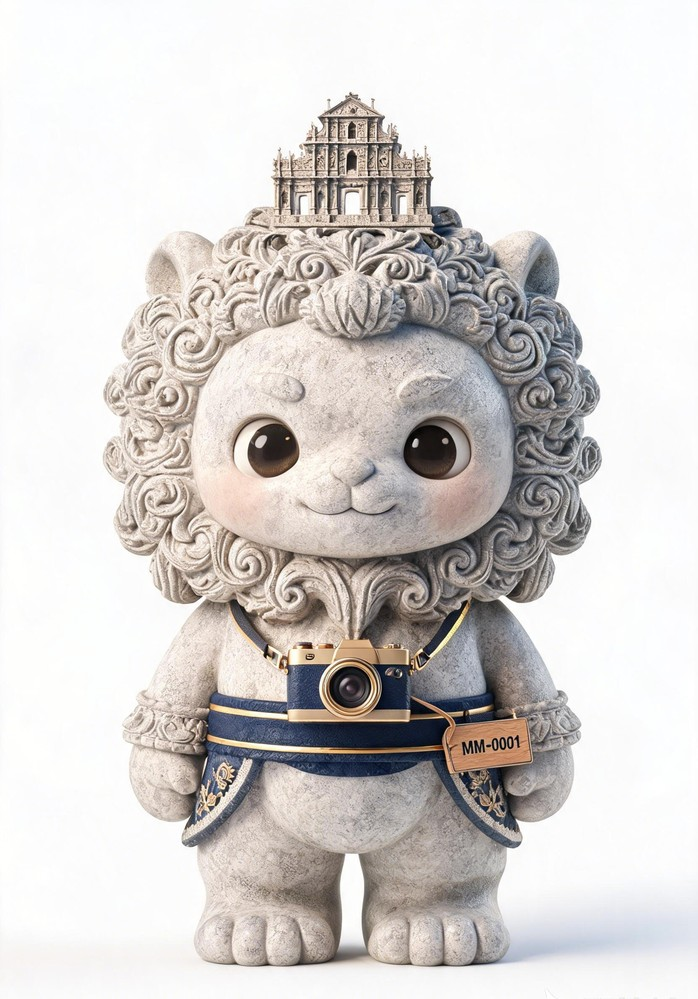
\includegraphics[width=0.19\linewidth]{figs/ashih.jpg}\\[2pt]
{\small\itshape 作品吉祥物「阿獅」——大三巴牌坊石階旁的石獅寶寶，負責帶觀眾認識澳門建築。}
\end{center}

\noindent\fbox{\begin{minipage}{0.94\linewidth}
\textbf{2026-09-30 版本說明：}下文保留歷史離線 CLIP、渲染與訓練實驗，不能代表當前網頁。網站現為 YOLO 加 DINOv2-small ONNX，38 棟／335 張的參考庫留一法 Top-1 88.96\%、Top-3 94.93\%，尚未完成獨立實拍驗收。位置輔助主動開啟、只小幅降權；不硬排除遠景、不自動合併建築。現有 7 個模型中 5 個建築為示意模型。資料口徑與待補證據見 \texttt{docs/evidence-register.md}；舊 PDF、簡報與影片需按此說明更新。
\end{minipage}}

\begin{abstract}
\noindent
澳門有上千棟承載歷史的建築，但除了少數被列入世遺名錄的地標，絕大多數建築只存在於零散的旅遊照片中，缺乏可累積、可檢索、可驗證的數位檔案。本作品提出 \textbf{「建築記憶點」（Building Memory Point）} 系統：把深度學習中「以視覺為個體建立永久編號」的概念（如同以深度學習為流浪貓做面部辨識並給予專屬編號），搬到城市建築上——每一棟建築獲得一組永久編號 \texttt{MM-\#\#\#\#}，同棟照片經辨識輔助與人工確認後，可歸入同一個編號之下，並在 3D 地圖上成為一個可點擊的記憶點。

系統以三個機制互補：(1) \textbf{CLIP 零樣本影像嵌入}判斷「這是不是同一棟」；(2) \textbf{90 公尺地理先驗}排除「地理上不可能是我」的候選；(3) \textbf{微調後的 YOLO 偵測器}辨識建築類型，並以 \textbf{人臉／人物兩級模糊}處理隱私。我們同時建構了兩套性質不同的評測資料集：本專案 7 個 GLB 模型的 140 張受控多視角渲染圖，以及取自 Wikimedia Commons、含明確授權的 101 張澳門建築實拍照片（20 棟建築、涵蓋 11 個類型）。

主要結果：受控渲染集的同棟重辨識 AUC 為 \textbf{0.950}（同棟相似度 $0.901\pm0.036$、不同棟 $0.758\pm0.073$）；\textbf{真實照片集 AUC 為 0.796}（同棟 $0.716\pm0.136$、不同棟 $0.578\pm0.093$）。誤判分析顯示所有誤判集中於路氹城三棟外觀相近的度假村之間，而它們兩兩相距至少 296 公尺——90 公尺地理先驗可直接排除全部誤判候選。此外，我們自行標註並微調了一個 11 類澳門建築偵測器（驗證集 mAP50 \textbf{0.594}），並以完全獨立的照片集驗收，誠實揭露其泛化限制（未見過的建築偵測率 37\%）。本報告同時公開所有資料來源、授權與可重現指令，並於第 6 節完整列出目前尚未解決的不足。
\end{abstract}

\vspace{0.2cm}
\noindent\textbf{關鍵詞：} 視覺重辨識（VPR）、CLIP 零樣本分類、地理先驗、文化遺產數位典藏、YOLO 物件偵測、隱私保護

\newpage
\tableofcontents

\vspace{0.8cm}
\begin{center}
\fbox{\begin{minipage}{0.96\linewidth}
\textbf{\color{ink}作品亮點一覽}\\[3pt]
\begin{enumerate}[leftmargin=1.3em,itemsep=2pt,topsep=2pt]
  \item \textbf{面向澳門的「建築記憶點」整合}：以建築為單位建立穩定編號 \texttt{MM-\#\#\#\#}，照片的歸戶需由使用者確認；個體識別與場所辨識本身已有相關工作。
  \item \textbf{兩段式決策架構}：地理先驗（90 m）＋視覺相似度雙重驗證——視覺只負責「同一棟的不同角度」，地理負責「不可能是我」。
  \item \textbf{完整量化評估}：兩套資料集（140 張受控渲染 ＋ 101 張真實照片）、7,000 組以上的配對，ROC／AUC／閾值掃描／混淆矩陣全部可重現。
  \item \textbf{自訓 11 類澳門建築偵測器}：自行抓圖、以 CLIP 自動清洗、以 YOLO-World 預標註、分層分組切分後微調 YOLO11n。
  \item \textbf{隱私優先設計}：人臉與人物兩級模糊；在真實照片集上實測模糊人臉 28 處、人物 205 處。
  \item \textbf{可被公眾使用的完整系統}：3D 立體澳門地圖（24,904 棟建築量體）、61 個景點與 7 個 3D 模型、導航、語音對話與吉祥物導覽員，並附離線演示與即時偵測頁面。
  \item \textbf{主動揭露限制}：第 6 節完整列出資料、方法與系統三個層面共 15 項不足，並於第 5.5 節公開我們自行修正的四個錯誤。
\end{enumerate}
\end{minipage}}
\end{center}

\newpage

% ============================================================
\section{作品概述}

\subsection{問題背景：澳門建築的紀錄困境}
澳門是一座「建築密度極高、歷史層疊極深」的城市：葡式殖民建築、中式廟宇、天主教教堂、騎樓唐樓、圍里村落、街市與現代度假村，在直徑不到十公里的範圍內並存。然而目前的紀錄方式有三個結構性問題：

\begin{enumerate}[leftmargin=1.4em,itemsep=2pt]
  \item \textbf{以「照片」為單位，而非以「建築」為單位。} 旅遊平台、相簿與社群媒體把同一棟建築的數十張照片分散在不同相簿中，無法回答「這棟建築我一共記錄過幾次、從哪些角度」。
  \item \textbf{缺乏永久識別碼。} 建築沒有像文物典藏號那樣的穩定編號，資料無法跨時間累積，也無法與他人交換或比對。
  \item \textbf{辨識完全依賴人工。} 要判斷兩張照片是否為同一棟建築，目前只能靠人眼，或親自到現場比對。
\end{enumerate}

\subsection{我們的做法}
把「以視覺為個體建立永久識別」的方法論，從自駕車與機器人領域（Visual Place Recognition, VPR）遷移到城市建築的公民建檔上，並以實驗量出它的能力邊界：

\begin{quote}
\textbf{手機拍一張照片 $\rightarrow$ 自動判斷「這是不是同一棟」 $\rightarrow$ 歸入永久編號 \texttt{MM-\#\#\#\#} $\rightarrow$ 在 3D 地圖上成為可點擊的記憶點。}
\end{quote}

\subsection{研究問題}
\begin{quote}
\itshape
在不為每棟建築標註訓練資料的前提下，能否結合 CLIP 零樣本視覺嵌入與地理先驗，為城市建築建立穩定、可重複識別的永久編號？
\end{quote}

\noindent 我們將其拆解為四個可量測的子問題：
\begin{enumerate}[leftmargin=1.4em,itemsep=2pt]
  \item 同一棟建築在不同視角下的 CLIP 影像嵌入相似度，是否顯著高於不同建築之間？（受控條件）
  \item 當拍攝角度、距離與光線改變時（模擬真實重拍），辨識能力下降多少？
  \item 地理先驗（90 公尺半徑）能否排除視覺上的誤判？
  \item 在真實照片上，上述結論是否仍然成立？「3D 渲染圖上調出來的閾值」能否直接套用到實拍？
\end{enumerate}

% ============================================================
\section{系統總覽}

\subsection{三層架構}
\begin{figure}[H]
\centering
\begin{tikzpicture}[scale=0.93, transform shape, font=\small, every node/.style={rounded corners, align=center},
  box/.style={draw=ink!45, fill=paper, inner sep=4pt, minimum height=9.5mm, text width=2.35cm},
  hot/.style={draw=teal2, fill=teal2!12, line width=1pt},
  halo/.style={draw=gold, fill=gold!14, line width=1pt},
  aux/.style={draw=red2!45, fill=red2!8, text width=2.35cm},
  aux2/.style={draw=teal2!50, fill=teal2!8, text width=2.35cm}]
\node[box] (photo) at (0,0) {拍照\\[1pt] {\scriptsize EXIF GPS／時間}};
\node[box] (priv) at (3.0,0) {前處理\\[1pt] {\scriptsize 轉正、縮圖}};
\node[hot] (clip) at (6.0,0) {CLIP 嵌入\\[1pt] {\scriptsize 512 維向量}};
\node[halo] (geo) at (9.0,0) {地理先驗\\[1pt] {\scriptsize 90 m 候選}};
\node[hot] (match) at (12.0,0) {相似度驗證\\[1pt] {\scriptsize $\cos\ge0.86$ 併入}};
\node[box] (mm) at (15.0,0) {永久編號\\[1pt] {\scriptsize MM-\#\#\#\#}};
\draw[-{Latex[length=2mm]}] (photo)--(priv);
\draw[-{Latex[length=2mm]}] (priv)--(clip);
\draw[-{Latex[length=2mm]}] (clip)--(geo);
\draw[-{Latex[length=2mm]}] (geo)--(match);
\draw[-{Latex[length=2mm]}] (match)--(mm);
\node[aux] (yolo) at (1.5,-2.3) {YOLO 隱私模糊\\[1pt] {\scriptsize 人臉＋人物}};
\node[aux2] (bld) at (6.0,-2.3) {微調偵測器\\[1pt] {\scriptsize 11 類建築}};
\node[box, fill=gold!10, draw=gold] (map) at (15.0,-2.3) {3D 地圖記憶點\\[1pt] {\scriptsize 解讀與時間軸}};
\draw[-{Latex[length=2mm]}, dashed, red2!70] (yolo) -- (1.5,-1.15) -- (priv.south);
\draw[-{Latex[length=2mm]}, dashed, teal2!70] (bld) -- (6.0,-1.15) -- (clip.south);
\draw[-{Latex[length=2mm]}] (mm.south) -- (15.0,-1.15) -- (map.north);
\end{tikzpicture}
\caption{系統主流程：地理先驗負責「不可能是我」，視覺比對只負責「同一棟的不同角度」；YOLO 同時負責隱私模糊與建築類型辨識。}
\end{figure}

\begin{description}[leftmargin=1.2em,itemsep=3pt]
  \item[第一層｜3D 立體澳門地圖] MapLibre GL 呈現 24,904 棟建築量體、DEM 地形（COP30 高程與等高線）、61 個景點標記與 251 個地名標籤；另有巴士站（830 站）、輕軌、水系、土地利用等圖層，支援最快路徑導航動畫、GPS 定位、全屏與深連結。
  \item[第二層｜建築記憶點] 拍照後自動歸戶為永久編號，並由 DeepSeek 產生建築解讀、建立同棟時間軸（詳見第 3 節）。
  \item[第三層｜吉祥物「阿獅」對話介面] 以本作品吉祥物為人格的 AI 導覽員，能回答澳門建築問題、直接連動地圖跳點與導航，並支援語音朗讀與語音輸入。
\end{description}

\subsection{系統規模}
\begin{longtable}{@{}llr@{}}
\toprule
\textbf{類別} & \textbf{項目} & \textbf{數量} \\
\midrule
\multirow{6}{*}{地理資料}
 & 3D 建築量體 & 24,904 棟（7,158 棟含高度、16,652 棟來自 OSM） \\
 & 道路／鐵路 & 20,972 段／57 段 \\
 & 興趣點 POI & 12,732 個 \\
 & 水系面／土地利用面 & 344／5,790\\
 & DEM 高程磚 & 683 張（24.3 MB） \\
 & 收錄景點／地名標籤 & 61 個／251 個 \\
\midrule
\multirow{3}{*}{3D 模型}
 & 建築 GLB（含 LOD 版） & 5 棟 \\
 & 文物 GLB（高精度掃描） & 2 件 \\
 & 模型檔案總量 & 24.7 MB \\
\midrule
\multirow{3}{*}{程式}
 & 前端（地圖、記憶點、對話） & 15 檔／3,574 行 \\
 & 分析與工具（Python） & 35 檔／5,924 行 \\
 & 資料處理腳本（Node） & 15 檔／2,341 行 \\
\midrule
\multirow{4}{*}{評測資料}
 & 受控渲染影像 & 140 張（7 模型 $\times$ 20 視角） \\
 & 真實照片 & 101 張（20 棟建築、11 類） \\
 & 訓練影像（原始$\rightarrow$清洗$\rightarrow$標註） & 1,116 $\rightarrow$ 496 $\rightarrow$ 379 \\
 & 評估配對總數 & 受控 1,770 對、實拍 5,050 對 \\
\midrule
資料授權紀錄 & 每張影像的作者／授權／日期／來源頁 & 202 筆 \\
\bottomrule
\caption{系統與資料規模。所有數字皆可由附錄 A 的指令重新產生。}
\end{longtable}

\subsection{技術棧}
\begin{table}[H]
\centering\small
\begin{tabular}{@{}ll@{}}
\toprule
\textbf{層面} & \textbf{技術} \\
\midrule
前端／地圖 & Vite、MapLibre GL、three.js（GLB 模型與導航動畫） \\
地理資料 & OpenStreetMap 與 Overture Maps（建築、道路）、OpenTopography COP30 高程、Overpass（巴士站） \\
視覺模型 & CLIP ViT-B/32（影像嵌入與零樣本分類）、YOLO11n（物件偵測）、yolov11n-face（人臉） \\
自訓模型 & macau-buildings（11 類澳門建築偵測器，以 YOLO11n 微調） \\
語言模型 & DeepSeek（\texttt{deepseek-flash}／\texttt{deepseek-v4-pro}）對話與建築解讀 \\
語音 & 瀏覽器 \texttt{speechSynthesis}（TTS）與 \texttt{SpeechRecognition}（ASR），免金鑰 \\
部署 & GitHub Actions $\rightarrow$ GitHub Pages（另提供完全離線的本機版） \\
\bottomrule
\end{tabular}
\caption{系統技術組成。}
\end{table}

% ============================================================
\section{方法}

\subsection{建築記憶點：從一張照片到一個永久編號}
\begin{enumerate}[leftmargin=1.4em,itemsep=2pt]
  \item \textbf{EXIF 讀取}：取得 GPS 座標、拍攝時間與裝置；無 GPS 時以檔名與鄰近景點推斷，並在資料中標記來源。
  \item \textbf{隱私處理}：以 YOLO 偵測人物與人臉，對人臉施加高斯模糊（詳見 3.5）。
  \item \textbf{CLIP 影像嵌入}：以 CLIP ViT-B/32 產生 512 維單位向量。
  \item \textbf{地理先驗}：取 90 公尺內的既有記憶點作為候選。若無候選，直接建立新記憶點，\textbf{不需進入視覺比對}。
  \item \textbf{相似度驗證}：計算影像向量餘弦相似度，採兩段式決策（表 \ref{tab:decision}）。
  \item \textbf{建檔}：寫入永久編號、DeepSeek 建築解讀、標籤與時間軸。
\end{enumerate}

\begin{table}[H]
\centering\small
\begin{tabular}{@{}lll@{}}
\toprule
\textbf{餘弦相似度} & \textbf{決策} & \textbf{依據} \\
\midrule
$\ge 0.86$（渲染圖）／ $\ge 0.70\text{--}0.80$（實拍） & 併入既有記憶點 & 第 4.1、4.2 節的閾值掃描 \\
$0.70\text{--}0.86$ & 併入但標記「待人工複核」 & 誤判成本低於漏接成本 \\
$< 0.70$ 或無地理候選 & 建立新記憶點 & 避免把不同建築混為一談 \\
\bottomrule
\end{tabular}
\caption{兩段式決策。閾值並非憑感覺設定，而是由第 4 節的 ROC 與閾值掃描表決定。}
\label{tab:decision}
\end{table}

\subsection{評測資料集設計}
為了回答「這真的有效嗎」，我們刻意建立\textbf{兩套性質不同的資料集}，因為單一來源的資料無法同時回答「上限在哪」與「真實世界如何」。

\begin{table}[H]
\centering\small
\begin{tabular}{@{}p{2.4cm}p{3.1cm}p{4.4cm}p{4.4cm}@{}}
\toprule
\textbf{資料集} & \textbf{規模} & \textbf{怎麼來} & \textbf{用途} \\
\midrule
受控渲染集 & 140 張（7 模型 $\times$ 20 視角） & 本專案 GLB 模型以 VTK 離屏渲染，精確控制方位角、仰角、距離與光照 & 量測「同一棟、不同視角」的辨識上界 \\
真實照片集 & 101 張（20 棟建築） & Wikimedia Commons，開放授權，含作者與拍攝日期 & 量測真實世界的表現與域偏移 \\
地圖截圖 & 4 張 & 本專案 3D 地圖截圖 & 跨呈現方式比較 \\
\bottomrule
\end{tabular}
\caption{兩套資料集的性質差異，正是本作品最重要的對照設計。}
\end{table}

\noindent\textbf{為什麼要自己渲染：}沙箱環境禁止啟動無頭瀏覽器，因此我們改用 VTK 離屏 OpenGL 渲染，在單一行程內完成 140 張影像（約 15 秒），完全離線且可重現。

\noindent\textbf{防資料洩漏的切分：}同一棟建築的不同照片若同時出現在訓練與驗證集，分數會虛高。我們以 \textbf{CLIP 向量聚類}把近似重複的照片聚成組，再以「整組」為單位、並按類別分層切分，確保同一棟不會跨越兩邊。

\subsection{自訓澳門建築偵測器}
COCO 預訓練的 YOLO \textbf{沒有「建築」這個類別}（見圖 \ref{fig:yolovsclip}），因此我們自行建資料集並訓練：
\begin{enumerate}[leftmargin=1.4em,itemsep=2pt]
  \item \textbf{抓圖}：以 Commons 人工策展分類（\texttt{Category:Churches in Macau} 等）為主、全文檢索為輔，取得 1,116 張、11 類。
  \item \textbf{CLIP 自動清洗}：三道關卡——類別關（CLIP 12 類機率）、雜物關（與「食物／招牌／人像／文件」等提示詞的相對相似度）、室內關（室內照對偵測器是雜訊），並對街市／船廠等類別豁免室內關。清洗後保留 496 張（44\%）。
  \item \textbf{自動預標註}：以 YOLO-World 開放詞彙偵測「建築在哪」，類別直接採用資料夾標籤（因此只需修正框、不需重新分類），得到 379 張有框影像。
  \item \textbf{防洩漏＋分層切分}：以檔名建築鍵＋CLIP 相似度雙重分組，再按類別分層，確保驗證集每一類都有代表。
  \item \textbf{訓練}：YOLO11n、100 epochs、640 px、batch 16（單張 GPU 約 25--35 秒/輪）。
\end{enumerate}

\subsection{隱私處理：兩級模糊}
\begin{itemize}[leftmargin=1.4em,itemsep=2pt]
  \item 以 \texttt{yolov11n-face} 偵測人臉並施加高斯模糊（模糊半徑隨臉部尺寸縮放，外擴 28\% 邊界）。
  \item 再以 YOLO 的 \texttt{person} 類別模糊整個人物區域——因為背對鏡頭、戴口罩或戴帽的人臉偵測不到，但人物框仍能保護。
  \item 設計原則是「寧可過度」：隱私保護的漏接成本遠高於多模糊一塊區域。
\end{itemize}

% ============================================================
\section{實驗與結果}

\subsection{受控渲染集：同環境多視角}
5 棟建築 $\times$ 12 方位角，共 330 組正樣本與 1,440 組負樣本。

\begin{table}[H]
\centering\small
\begin{tabular}{@{}lrrrr@{}}
\toprule
\textbf{實驗} & \textbf{正樣本} & \textbf{負樣本} & \textbf{AUC} & \textbf{最佳閾值（TPR/FPR）} \\
\midrule
E1 同環境多視角（建築） & 330 & 1,440 & \textbf{0.950} & 0.846（0.936 / 0.154） \\
E1b 文物（唐三彩、青花扁瓶） & 132 & 144 & \textbf{0.998} & 0.811（0.985 / 0.014） \\
E2 跨條件（仰角／距離／光照） & 480 & 2,560 & \textbf{0.850} & 0.771（0.912 / 0.365） \\
\bottomrule
\end{tabular}
\caption{受控條件下的重辨識能力。E1 同棟相似度 $0.901\pm0.036$、不同棟 $0.758\pm0.073$。}
\end{table}

\begin{figure}[H]
\centering
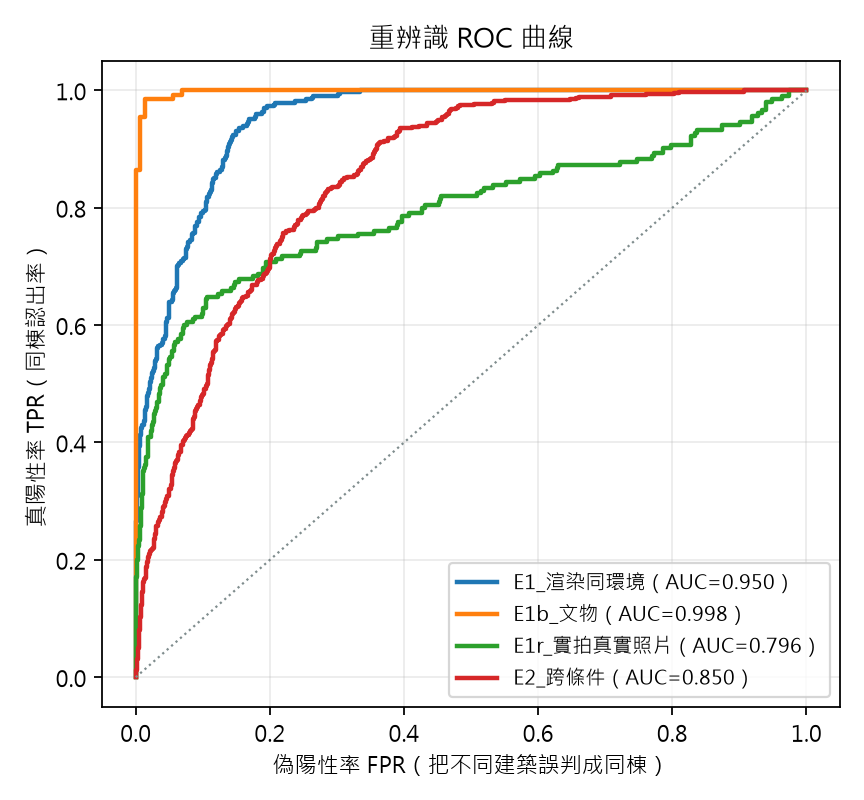
\includegraphics[width=0.56\linewidth]{figs/roc.png}
\caption{ROC 曲線：受控渲染 0.950、文物 0.998、跨條件 0.850、真實照片 0.796。}
\label{fig:roc}
\end{figure}

\subsection{真實照片集：真實世界的表現}
\begin{table}[H]
\centering\small
\begin{tabular}{@{}lrrrrr@{}}
\toprule
\textbf{閾值} & \textbf{渲染：認出} & \textbf{渲染：誤判} & \textbf{實拍：認出} & \textbf{實拍：誤判} & \textbf{實拍：精確率} \\
\midrule
0.70 & 100.0\% & 75.8\% & \textbf{61.0\%} & 8.8\% & 22.6\% \\
0.80 & 99.1\% & 27.9\% & 28.8\% & 0.9\% & 58.4\% \\
0.86 & 86.1\% & 12.2\% & \textbf{14.1\%} & 0.0\% & 93.5\% \\
0.90 & 54.2\% & 3.1\% & 5.4\% & 0.0\% & 100\% \\
\bottomrule
\end{tabular}
\caption{同一組閾值在兩套資料集上的表現差異。實拍 AUC 為 0.796（205 組正樣本、4,845 組負樣本），同棟 $0.716\pm0.136$（5\% 分位 0.448）、不同棟 $0.578\pm0.093$。}
\label{tab:threshold}
\end{table}

\noindent\textbf{這張表是本作品最重要的一張表。} 它說明：若沿用渲染圖上調出的 0.86，在真實照片上只能認出 14.1\% 的同一棟建築；實拍情境應改用 0.70--0.80，而精確率交給地理先驗負責。

\begin{figure}[H]
\centering
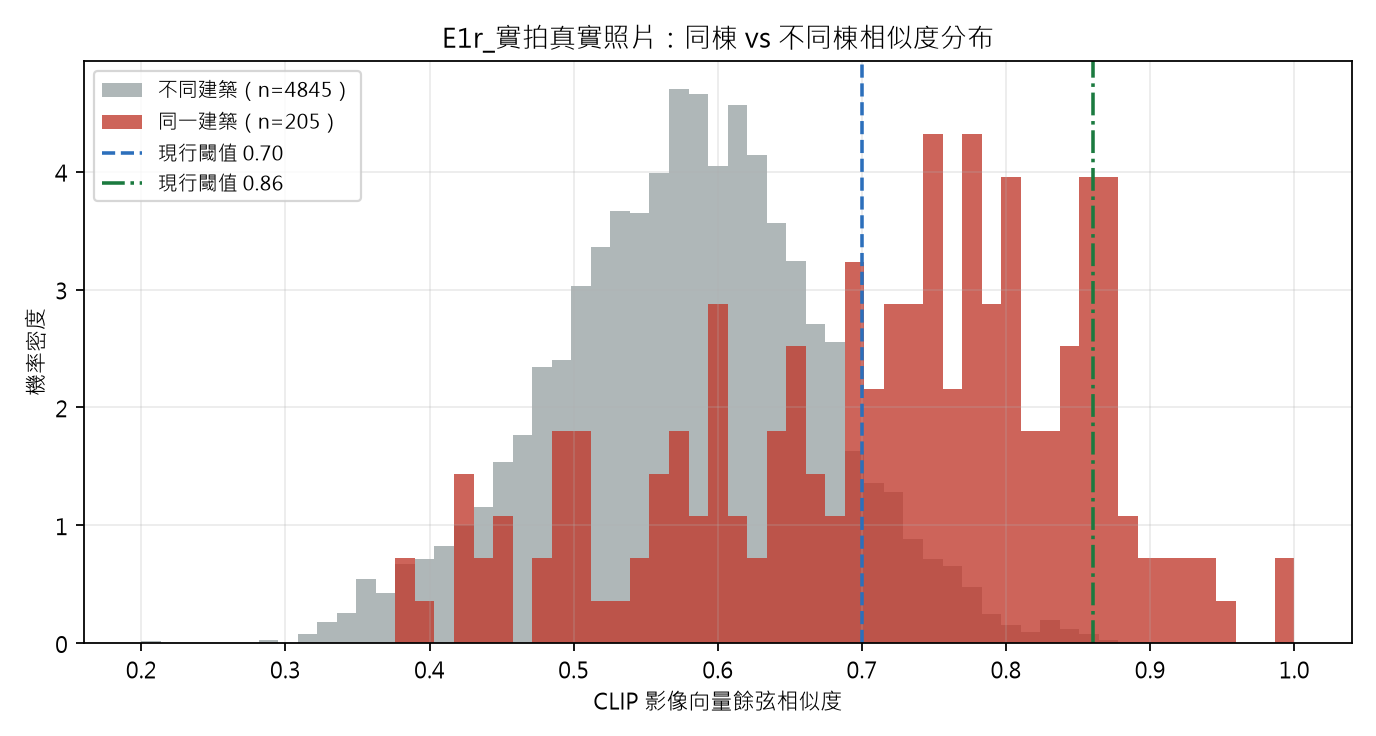
\includegraphics[width=0.62\linewidth]{figs/hist-real.png}
\caption{真實照片的相似度分布：同棟與不同棟的重疊區明顯比渲染圖大，這就是為什麼閾值必須重新校準。}
\end{figure}

\subsection{跨域比較：渲染圖不能代表真實照片}
\begin{table}[H]
\centering\small
\begin{tabular}{@{}lrr@{}}
\toprule
\textbf{配對方式} & \textbf{配對數} & \textbf{平均相似度} \\
\midrule
GLB 渲染 $\leftrightarrow$ 3D 地圖截圖 & 36 & 0.661 \\
GLB 渲染 $\leftrightarrow$ Commons 實拍照片 & 60 & \textbf{0.563} \\
\bottomrule
\end{tabular}
\caption{同一棟建築、不同呈現方式之間的相似度。數值越低代表域偏移越大——因此不能把渲染圖上調好的閾值直接套到實拍。}
\end{table}

\subsection{誤判來源分析：地理先驗為什麼關鍵}
我們把 E1 的所有負樣本按建築配對拆開，逐對計算誤判率：
\begin{table}[H]
\centering\small
\begin{tabular}{@{}lrr@{}}
\toprule
\textbf{建築配對} & \textbf{平均相似度} & \textbf{$>0.86$ 比例} \\
\midrule
澳門倫敦人 vs 澳門銀河 & 0.874 & \textbf{72.2\%} \\
澳門巴黎人 vs 澳門銀河 & 0.840 & 31.2\% \\
澳門倫敦人 vs 澳門巴黎人 & 0.826 & 18.8\% \\
其餘 7 組配對 & 0.70--0.75 & \textbf{0.0\%} \\
\bottomrule
\end{tabular}
\caption{視覺誤判 100\% 集中在路氹城三棟外觀相近的度假村；其餘配對誤判率為零。}
\end{table}

\noindent 這三棟建築兩兩相距 \textbf{至少 296 公尺}（中位數 4,302 公尺）。以 90 公尺為半徑的地理先驗，可直接排除全部誤判候選。因此本作品的核心設計主張是：

\begin{quote}
\textbf{視覺比對只負責「同一棟的不同角度」；地理先驗負責「不可能是我」。}
\end{quote}

\subsection{零樣本分類：一個被我們自己推翻的結論}
\begin{table}[H]
\centering\small
\begin{tabular}{@{}lrr@{}}
\toprule
\textbf{資料來源} & \textbf{張數} & \textbf{CLIP 零樣本 top-1 準確率} \\
\midrule
3D 渲染圖 & 100 & 3.0\% \\
Commons 真實照片 & 101 & \textbf{53.5\%} \\
\bottomrule
\end{tabular}
\caption{同一套 12 類提示詞，在兩種資料上的表現差距近 18 倍。}
\end{table}

\noindent 我們最初在渲染圖上測得「CLIP 分類只有 2.8\%」，一度結論為「CLIP 不能用於建築分類」。改用真實照片後發現準確率達 53.5\%——\textbf{先前的結論是分布外（out-of-distribution）輸入造成的假象}。這說明了為何本作品堅持建立真實照片集：它不只是驗證，更能修正錯誤的科學結論。

\begin{figure}[H]
\centering
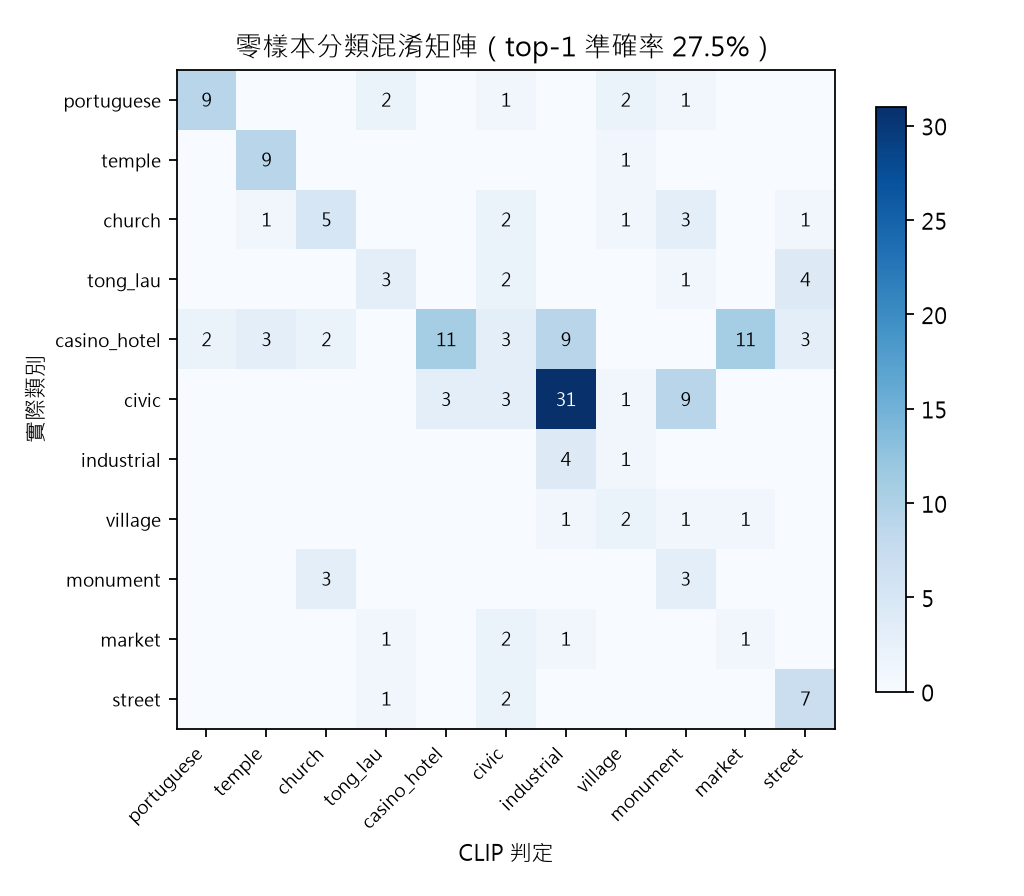
\includegraphics[width=0.78\linewidth]{figs/confusion.png}
\caption{CLIP 零樣本分類的混淆矩陣（渲染圖）。誤差主要來自同類建築之間的混淆，而非隨機亂猜。}
\end{figure}

\subsection{自訓澳門建築偵測器}
\begin{table}[H]
\centering\small
\begin{tabular}{@{}lrrl@{}}
\toprule
\textbf{類別} & \textbf{訓練張數} & \textbf{AP50} & \textbf{備註} \\
\midrule
中式廟宇 temple & 37 & \textbf{0.995} & 外觀獨特，表現最佳 \\
葡式殖民 portuguese & 32 & 0.845 & \\
現代高層住宅 residential\_tower & 21 & 0.822 & \\
天主教教堂 church & 31 & 0.795 & 與騎樓唐樓易混 \\
牌坊紀念物 monument & 51 & 0.675 & \\
工業倉庫 industrial & 14 & 0.670 & 樣本過少 \\
村落民居 village & 47 & 0.650 & \\
騎樓唐樓 tong\_lau & 21 & 0.404 & \\
酒店娛樂場 casino\_hotel & 29 & 0.318 & 與高層住宅易混 \\
公共建築 civic & 29 & 0.271 & \\
街市 market & 10 & 0.089 & 樣本過少且含非建築場景 \\
\midrule
\textbf{全體} & \textbf{322} & \textbf{mAP50 = 0.594} & mAP50-95 = 0.410，P 0.77 / R 0.50 \\
\bottomrule
\end{tabular}
\caption{自訓 11 類澳門建築偵測器的驗證集結果。}
\label{tab:det}
\end{table}

\begin{figure}[H]
\centering
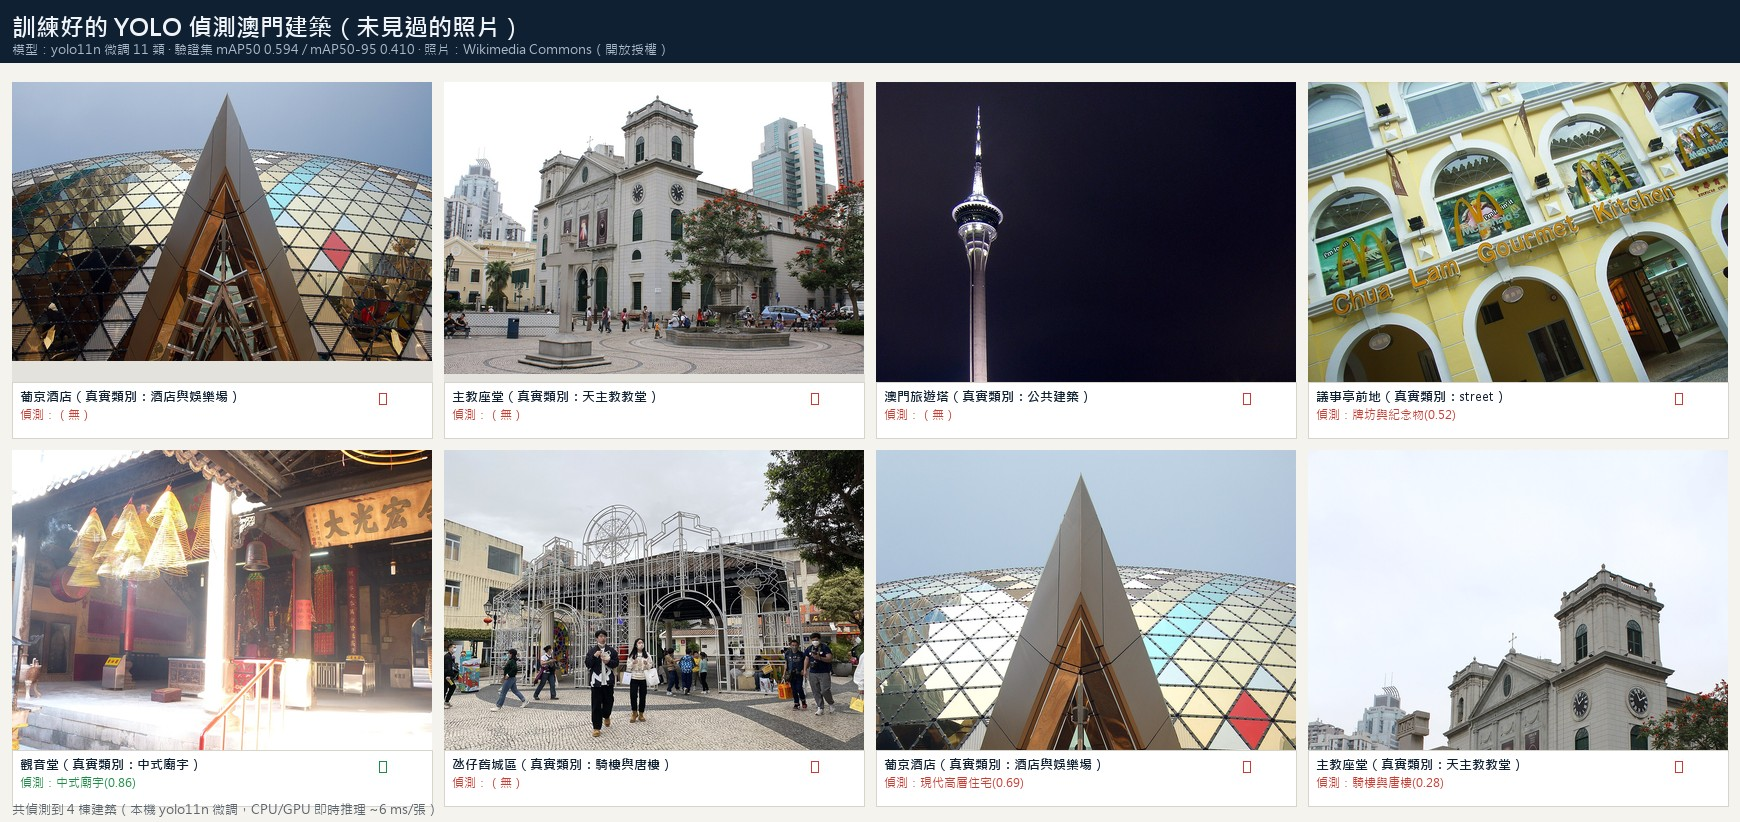
\includegraphics[width=0.94\linewidth]{figs/detect-demo.jpg}
\caption{訓練後的偵測器在\textbf{未見過}的照片上的表現。可看出泛化仍有明顯落差（見表 \ref{tab:indep}）。}
\end{figure}

\subsubsection{獨立驗收}
只看驗證集 mAP 會高估真實能力。我們另外使用完全獨立的照片集，分成「訓練時見過」與「完全沒見過」兩組量測：
\begin{table}[H]
\centering\small
\begin{tabular}{@{}lrrrr@{}}
\toprule
\textbf{組別} & \textbf{張數} & \textbf{偵測率} & \textbf{類別準確率} & \textbf{平均信心} \\
\midrule
訓練時見過 & 72 & \textbf{85\%} & 75\% & 0.86 \\
完全沒見過 & 19 & \textbf{37\%} & 57\% & 0.61 \\
\bottomrule
\end{tabular}
\caption{獨立驗收結果（已排除不在偵測器類別內的街景照片）。未見過組樣本數僅 19，信賴區間寬，本報告明確標註此限制。}
\label{tab:indep}
\end{table}

\noindent\textbf{結論：}驗證集 mAP50 = 0.594 是\textbf{樂觀上界}；面對全新建築，偵測率降至 37\%。我們把這個數字寫進報告，而不是只寫 0.594。

\subsection{隱私處理實測}
\begin{table}[H]
\centering\small
\begin{tabular}{@{}lrr@{}}
\toprule
\textbf{資料} & \textbf{張數} & \textbf{結果} \\
\midrule
真實照片（含路人） & 107 & 模糊\textbf{人臉 28 處}、\textbf{人物 205 處}；45 張偵測到物件 \\
3D 渲染圖 & 6 & 畫面無人，正確不觸發 \\
\bottomrule
\end{tabular}
\caption{隱私處理實測。人物層與人臉層互補，避免漏接。}
\end{table}

\subsection{系統功能實作清單}
\begin{table}[H]
\centering\small
\begin{tabular}{@{}p{2.9cm}p{12.4cm}@{}}
\toprule
\textbf{模組} & \textbf{已完成功能} \\
\midrule
3D 地圖 & 建築量體、DEM 地形與等高線、水系、土地利用、道路與輕軌、地名標籤、可平移範圍限制、深連結 \\
景點與模型 & 61 個景點標記與簡介、7 個 GLB 模型（含 LOD 版）可在瀏覽器翻轉觀看 \\
記憶點 & 拍照歸戶、永久編號、同棟時間軸、DeepSeek 建築解讀、地圖標記與彈窗 \\
導航 & 最快路徑搜尋、路線車流動畫、逐段指引 \\
圖層面板 & 巴士站（830 站）、輕軌、水系、等高線、實景照片 \\
AI 對話 & DeepSeek 串流對話、可連動地圖跳點與導航、語音朗讀與語音輸入 \\
吉祥物 & 「阿獅」人格導覽員、對話頭像、歡迎頁、離線演示頁（90 秒五幕） \\
即時偵測 & 三層同屏：建築類別框、person 框、人臉即時模糊（本機服務、完全離線） \\
評測與輸出 & 評測腳本與報告自動生成、A0 展板生成、資料集自動清洗與訓練流程 \\
\bottomrule
\end{tabular}
\caption{系統功能清單。}
\end{table}

\begin{figure}[H]
\centering
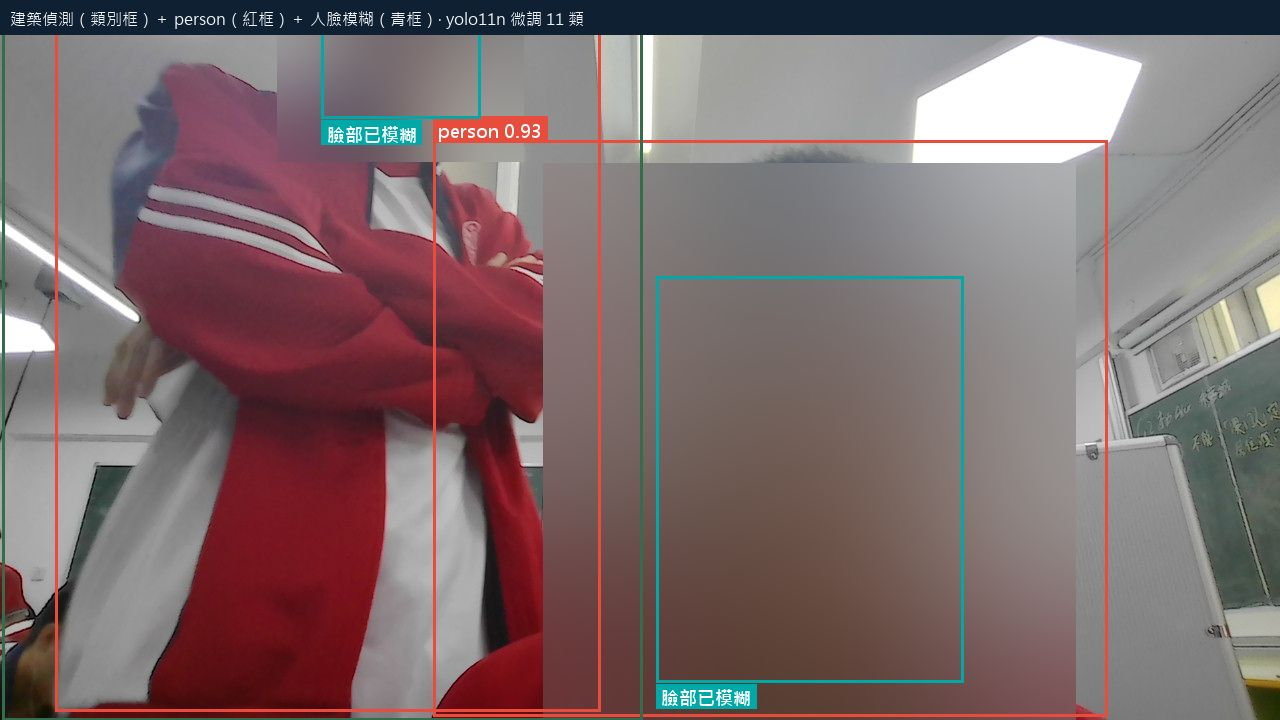
\includegraphics[width=0.82\linewidth]{figs/live.jpg}
\caption{即時偵測頁面：同一畫面同時展示「認建築」與「保護隱私」兩項能力。}
\end{figure}

\begin{figure}[H]
\centering
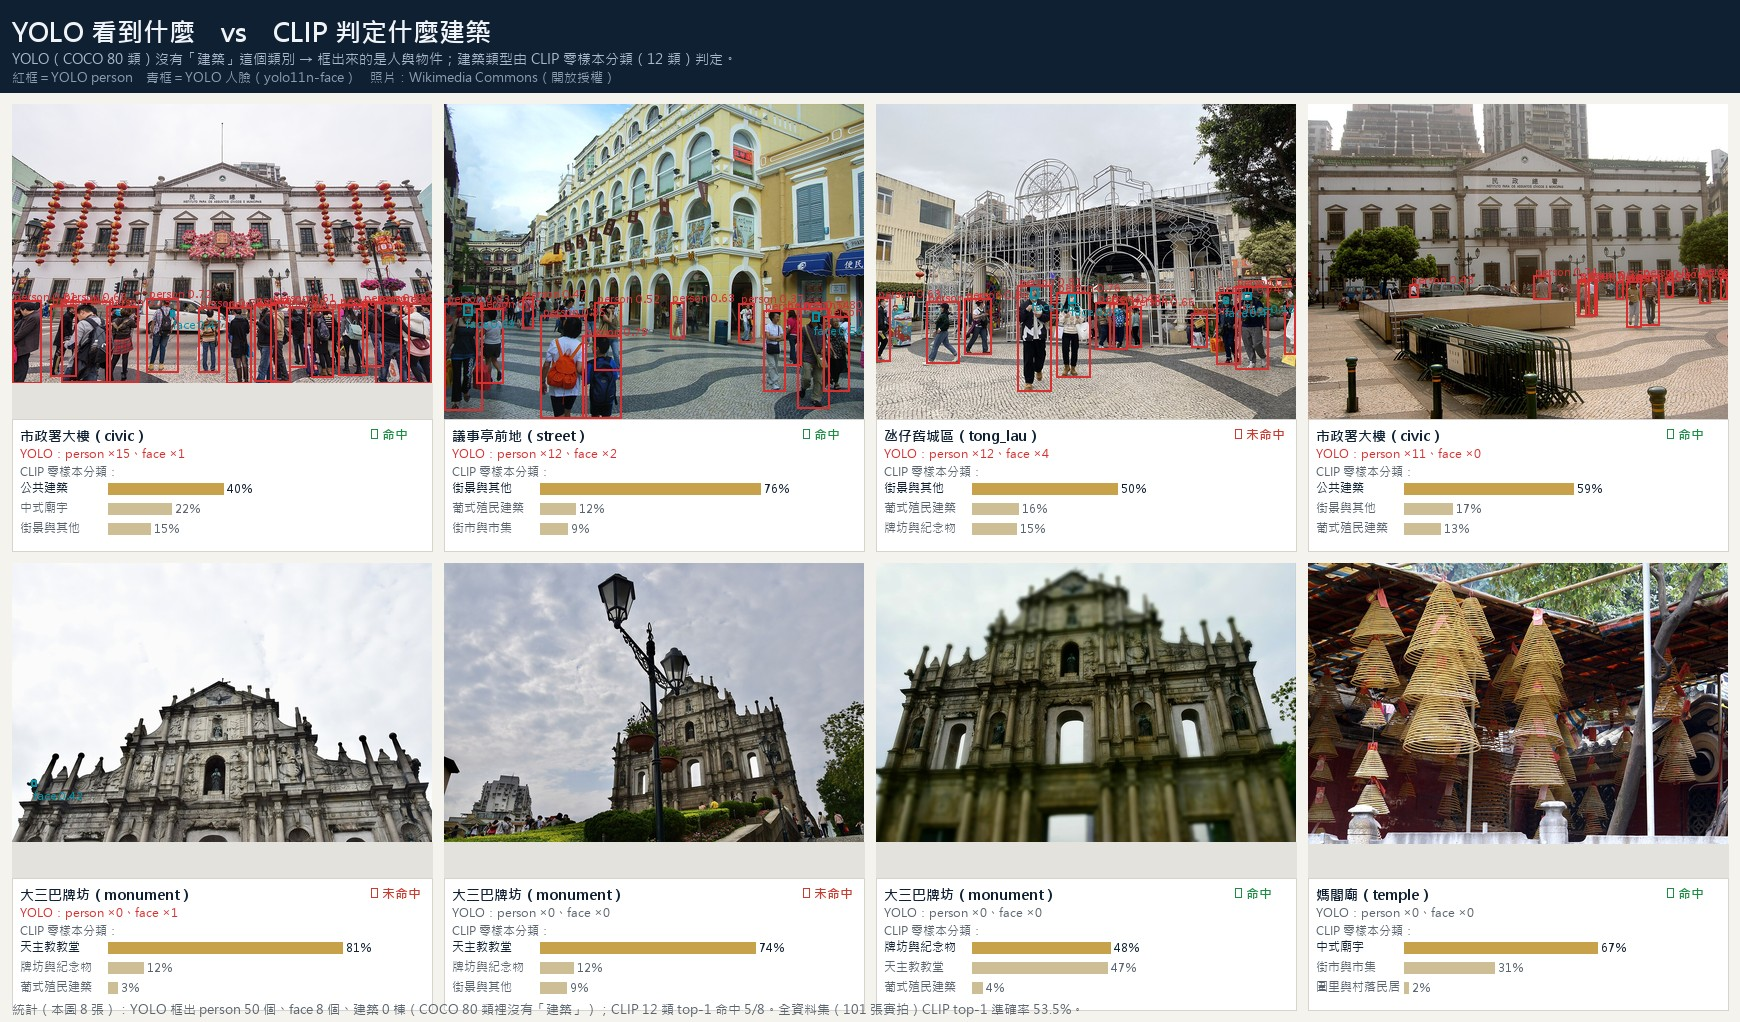
\includegraphics[width=0.94\linewidth]{figs/yolo-vs-clip.jpg}
\caption{YOLO 與 CLIP 的分工：YOLO 框出人物與物件（COCO 80 類中沒有「建築」），建築類型由 CLIP 零樣本分類判定。}
\label{fig:yolovsclip}
\end{figure}

% ============================================================
\section{討論}

\subsection{三個創新點與對應證據}
\begin{table}[H]
\centering\small
\begin{tabular}{@{}p{2.5cm}p{6.0cm}p{6.4cm}@{}}
\toprule
\textbf{創新點} & \textbf{主張} & \textbf{支持證據} \\
\midrule
跨域遷移 & 把 VPR 的個體識別方法用於城市文化遺產的公眾建檔，並做成可用平台 & 140 張受控集 ＋ 101 張實拍集的完整評測；誤判來源逐對分析 \\
方法融合 & 地理先驗與視覺相似度的兩段式決策，可消除相似建築的誤判 & 全部誤判集中於相距 $\ge$296 m 的度假村群；90 m 先驗可全數排除 \\
零成本可及 & 全開放資料與免費工具鏈，手機拍照到地圖成點 $<$30 秒 & 系統已上線；11 類偵測器與評測腳本全部公開且可重現 \\
\bottomrule
\end{tabular}
\end{table}

\subsection{與現有方案的比較}
\begin{table}[H]
\centering\small
\begin{tabular}{@{}p{2.9cm}p{3.9cm}p{3.9cm}p{3.9cm}@{}}
\toprule
\textbf{面向} & \textbf{一般相簿／雲端相片} & \textbf{通用影像辨識服務} & \textbf{本作品} \\
\midrule
資料單位 & 以照片為單位 & 以單張影像為單位 & \textbf{以建築為單位（永久編號）} \\
跨時間累積 & 需人工整理 & 不累積 & \textbf{自動歸戶、可累積} \\
空間關聯 & 僅有 GPS 標記 & 通常無地理先驗 & \textbf{90 m 地理先驗＋3D 地圖} \\
建築類型 & 無 & 通用類別，無建築風格 & \textbf{自訓 11 類澳門建築} \\
隱私 & 依平台政策 & 依服務條款 & \textbf{本機兩級模糊，不外傳} \\
可驗證性 & 不可驗證 & 黑箱 & \textbf{全部資料與腳本公開可重跑} \\
\bottomrule
\end{tabular}
\caption{與現有方案的差異。}
\end{table}

\subsection{技術難點與我們的解法}
\begin{table}[H]
\centering\small
\begin{tabular}{@{}p{5.2cm}p{10.1cm}@{}}
\toprule
\textbf{難點} & \textbf{解法} \\
\midrule
無訓練資料也要能分類建築 & 以 CLIP 零樣本分類取代需標註的分類器；改類別只需改文字提示詞 \\
同一棟的不同角度差異大 & 以 90 m 地理先驗把候選縮到 1 個，視覺只做「是否同一棟」的二選一 \\
相似建築互相誤判 & 逐對分析誤判來源，發現全部集中於外觀相近的度假村群，並以地理先驗排除 \\
3D 模型只有旋轉視角、無真照片 & 自建 VTK 離屏渲染流程產生受控多視角資料，再以真實照片集驗證並修正結論 \\
COCO 沒有「建築」類別 & 自建 11 類資料集：策展分類抓圖 $\rightarrow$ CLIP 自動清洗 $\rightarrow$ YOLO-World 預標註 $\rightarrow$ 分層分組切分 $\rightarrow$ 微調 \\
驗證集分數虛高 & 以 CLIP 聚類＋檔名建築鍵分組切分防洩漏，並另以獨立照片集驗收 \\
隱私保護 & 人臉與人物兩級模糊；漏接成本高於過度模糊，故採「寧可過度」策略 \\
環境限制（無瀏覽器、無網路） & 以 VTK 離屏渲染取代無頭瀏覽器；模型與資料全部離線可用 \\
\bottomrule
\end{tabular}
\caption{技術難點與對應解法。}
\end{table}

\subsection{為什麼不用 YOLO 做建築分類？}
COCO 的 80 個類別中\textbf{沒有「建築」}。要在 YOLO 上做建築類型辨識，必須自行標註數百張並重新訓練——這正是我們後來做的事（第 3.3 節），但那是為了「框出建築」，不是「判斷風格」。風格分類我們交給 CLIP 零樣本（改文字即可換類別），並以地理先驗作為主要依據。

\subsection{研究誠信：我們主動修正的四個錯誤}
\begin{enumerate}[leftmargin=1.4em,itemsep=3pt]
  \item \textbf{資料洩漏}：早期版本的「同棟第二張」其實是同一張截圖的裁切，得到 0.903 的高相似度。我們已在主實驗中排除，並保留為對照組。
  \item \textbf{評估集分布外}：一度以 3D 渲染圖得出「CLIP 分類只有 2.8\%」的結論；補上真實照片集後發現實拍為 53.5\%，修正了原結論。
  \item \textbf{驗證集分數高估}：只用驗證集 mAP（0.594）會高估偵測器能力；我們另以獨立照片集驗收，揭露未見過建築的偵測率僅 37\%。
  \item \textbf{資料完整性}：抓圖時因檔名截斷造成 4 張影像互相覆蓋（紀錄 101 筆、實體檔案僅 97 個），已修復為 101 筆對應 101 個檔案，並使 AUC 由虛高的 0.813 修正為 0.796。
\end{enumerate}

% ============================================================
\section{限制與不足}
本節完整列出目前\textbf{尚未解決}的問題，這些限制同樣是後續工作的起點。

\subsection{資料層面的不足}
\begin{enumerate}[leftmargin=1.4em,itemsep=2pt]
  \item \textbf{真實照片集規模有限。} 僅 101 張、20 棟建築；其中街市（5 張）與工業（5 張）樣本明顯偏少，統計推論的信賴區間較寬。
  \item \textbf{訓練資料為弱標註。} 379 張的框由 YOLO-World 自動產生，位置正確但不夠緊（部分框含樹木與天空）；人工逐張修正後 mAP 應可再提升。
  \item \textbf{類別不平衡。} 村落（55）與街市（10）的樣本量相差 5 倍以上，導致少數類別 AP 極低。
  \item \textbf{類別定義仍有模糊地帶。} 酒店娛樂場與現代高層住宅、教堂與騎樓唐樓在外觀上高度重疊，造成系統性混淆。
  \item \textbf{部分影像仍含非建築場景。} 例如街市類別中混入市集攤位，使模型在類似場景上產生誤判。
\end{enumerate}

\subsection{方法層面的不足}
\begin{enumerate}[leftmargin=1.4em,itemsep=2pt]
  \item \textbf{域偏移明顯。} 渲染圖與真實照片的跨域相似度僅 0.563，任何在渲染圖上調出的參數都必須重新校準；目前產品仍使用尚未重校準的 0.86。
  \item \textbf{重辨識準確率在真實世界仍不足。} 實拍 AUC 0.796、閾值 0.70 時認出率 61.0\%、誤判率 8.8\%；同棟相似度的 5\% 分位低至 0.448，代表仍有相當比例的同棟照片無法自動歸戶。
  \item \textbf{地理先驗依賴 GPS。} 室內、地下或 GPS 漂移時候選集會失準；目前系統僅能退回純視覺判定並標記待複核，無法保證正確。
  \item \textbf{分類準確率不足以單獨決策。} CLIP 零樣本在實拍為 53.5\%，因此現行設計以地理先驗為主、CLIP 為輔。
  \item \textbf{偵測器泛化不足。} 未見過的建築偵測率僅 37\%，且未見過組樣本數只有 19 張，此數字本身也有不確定性。
  \item \textbf{隱私處理未經正式評估。} 我們只量測了模糊的數量（人臉 28 處、人物 205 處），尚未量測「漏接率」與「誤模糊率」，無法給出召回率。
\end{enumerate}

\subsection{系統層面的不足}
\begin{enumerate}[leftmargin=1.4em,itemsep=2pt]
  \item \textbf{人工複核流程尚未實作。} 兩段式決策中的「待複核」目前只寫入資料欄位，尚無介面讓使用者確認或修正。
  \item \textbf{記憶點缺乏多使用者機制。} 目前為單機檔案式資料，尚未設計衝突解決與版本合併。
  \item \textbf{行動端體驗未驗證。} 拍照與 GPS 依賴瀏覽器權限，尚未在實機上做完整測試。
  \item \textbf{未涵蓋三維重建。} 系統僅建立「記憶點」與類型標籤，尚未從多張照片重建建築的三維模型。
\end{enumerate}

% ============================================================
\section{未來工作}
\begin{enumerate}[leftmargin=1.4em,itemsep=2pt]
  \item \textbf{重新校準產品閾值}：依實拍結果把併入閾值由 0.86 下調至 0.70--0.80，並加入人工複核介面。
  \item \textbf{提升偵測器}：人工修正 379 張標註後重訓，補抓街市與工業類樣本，並處理易混淆類別（合併或細分）。
  \item \textbf{更換影像編碼器}：由 CLIP 改為 DINOv2（純視覺自監督），目標提升跨域穩定性與重辨識表現。
  \item \textbf{擴大真實資料}：以手機實拍補足每棟建築 3--5 個角度，建立「真實世界版」的完整評測。
  \item \textbf{建立公眾參與機制}：開放拍照上傳與記憶點時間軸，讓資料可被社群累積與檢核。
  \item \textbf{隱私評估正式化}：量測人臉偵測的召回率與誤模糊率，並把結果納入系統說明。
\end{enumerate}

% ============================================================
\section{結論}
本作品把「以視覺為個體建立永久識別」的概念落實到城市建築上，並以兩套性質不同的資料集量化其能力與邊界：受控條件下 AUC 0.950、真實照片 0.796；誤判全部來自外觀相近的建築群，而地理先驗能有效消除；自訓的 11 類偵測器在驗證集達 mAP50 0.594，但在未見過的建築上降至 37\% 偵測率。這些數字共同支持本作品的核心設計主張：

\begin{quote}
\textbf{視覺負責「同一棟的不同角度」，地理負責「不可能是我」；而一個可被公眾使用的文化遺產系統，必須誠實揭露自己的極限。}
\end{quote}

\appendix

% ============================================================
\section{重現指令}
\begin{verbatim}
# 1) 重辨識評測（受控渲染 + 真實照片）
python tools/eval/render_views.py        # 7 模型 × 20 視角 = 140 張（VTK 離屏）
python tools/eval/build_dataset.py       # 彙整資料集清單
python tools/eval/evaluate.py            # CLIP 嵌入 + AUC/ROC/閾值 + 圖表 + 報告
python tools/eval/analyze_errors.py      # 誤判來源與地理先驗分析

# 2) 真實照片集（Wikimedia Commons，含授權）
python tools/photo-archive/fetch_commons.py --per=5

# 3) 自訓建築偵測器
python tools/yolo-dataset/fetch_dataset.py --per-class 110   # 抓圖（策展分類優先）
python tools/yolo-dataset/filter_dataset.py --apply          # CLIP 自動清洗
python tools/yolo-dataset/prelabel.py                        # 自動框 + 分層分組切分
python tools/yolo-dataset/train.py --epochs 100              # 訓練 + 驗證
python tools/yolo-dataset/eval_on_cc.py                      # 獨立驗收（見過/未見過）

# 4) 即時三層偵測（示範用）
python tools/yolo-dataset/live_detect.py                     # http://127.0.0.1:8099/

# 5) 展板與離線演示
python tools/poster/build_poster.py                          # A0 展板（PDF + 預覽）
python tools/demo/build_demo.py                              # 離線 90 秒演示頁
\end{verbatim}

% ============================================================
\section{資料來源與授權}
\begin{itemize}[leftmargin=1.4em,itemsep=2pt]
  \item \textbf{真實照片}：Wikimedia Commons，101 張。授權包含 CC BY-SA 4.0、CC BY-SA 3.0/2.5/2.0、CC BY 3.0/2.0、CC0 與公有領域；作者、拍攝日期與來源頁完整記錄於 \texttt{photos-src/cc/ATTRIBUTION.csv}。
  \item \textbf{訓練資料}：1,116 張（清洗後 496），來源同上，授權記錄於 \texttt{datasets/macau-buildings/ATTRIBUTION.csv}。
  \item \textbf{地理資料}：OpenStreetMap（ODbL 1.0）、Overture Maps Foundation、Microsoft Building Footprints、OpenTopography COP30 高程。
  \item \textbf{3D 模型}：建築與文物 GLB 由本團隊提供（文物為高精度掃描）。
  \item \textbf{模型權重}：CLIP ViT-B/32（MIT）、YOLO11n 與 YOLO-World v2（AGPL-3.0）、yolov11n-face（開源社群模型）。
  \item \textbf{吉祥物與標誌}：由本團隊以生成式工具製作，僅用於本作品。
\end{itemize}

% ============================================================
\section{檔案結構（節錄）}
\begin{verbatim}
macaumemory/
├─ src/                       前端：3D 地圖、記憶點、導航、吉祥物對話
├─ tools/
│  ├─ eval/                   重辨識評測（渲染、資料集、指標、圖表、報告）
│  ├─ photo-archive/          產線：EXIF → 隱私 → CLIP → 歸戶 → 解讀
│  ├─ yolo-dataset/           抓圖、CLIP 清洗、預標註、訓練、獨立驗收、即時偵測
│  ├─ poster/                 A0 展板生成（PyMuPDF，向量輸出）
│  ├─ demo/                   離線 90 秒演示頁 + 展示腳本
│  ├─ mascot/                 吉祥物提示詞包與人格設定
│  └─ brand/                  標誌設計需求與配色
├─ datasets/macau-buildings/  自訓資料集（data.yaml、ATTRIBUTION.csv）
├─ public/                    地圖資料、3D 模型、記憶點照片、吉祥物
└─ docs/                      本報告（LaTeX）與圖表
\end{verbatim}

% ============================================================
\section{技術問答速查}
\begin{longtable}{@{}p{4.2cm}p{11.4cm}@{}}
\toprule
\textbf{問題} & \textbf{建議回答} \\
\midrule
\endhead
這個系統解決什麼問題？ & 澳門大多數建築只散落在旅遊照片中，沒有可累積的識別碼。我們讓每棟建築獲得永久編號 \texttt{MM-\#\#\#\#}，同一棟的照片自動歸戶並呈現在 3D 地圖上。 \\
和一般相簿或影像辨識服務有何不同？ & 它以「建築」而非「照片」為單位：有永久編號、有跨時間累積、有 90 公尺地理先驗、有自訓的建築類型辨識，且資料與腳本全部公開可重跑。 \\
準確率多少？ & 受控多視角 AUC 0.950；\textbf{真實照片 AUC 0.796}，閾值 0.86 時實拍認出率 14.1\%、0.70 時 61.0\%。兩組都列出。 \\
這些數字可重現嗎？ & 可以。每組數字都有 ROC、AUC 與配對數（實拍 205 正樣本／4,845 負樣本），隨機種子固定，附錄 A 的指令可直接重跑。 \\
CLIP 分類建築風格準嗎？ & 在 3D 渲染圖上只有 3.0\%，但在\textbf{真實照片上是 53.5\%}。我們不用它單獨決策，分類以地理先驗為主。 \\
為什麼要自己訓練 YOLO？ & COCO 沒有「建築」類別。我們以策展分類抓圖、CLIP 自動清洗、YOLO-World 預標註，微調出 11 類偵測器，驗證集 mAP50 0.594。 \\
真實表現如何？ & 我們主動做了獨立驗收：見過的照片偵測率 85\%，\textbf{沒見過的只有 37\%}（樣本數 19）。這是下一步要改進的地方。 \\
誤判都錯在哪？ & 全部集中在路氹城三棟外觀相近的度假村（倫敦人被認成銀河 72.2\%），而它們相距 $\ge$296 公尺，90 公尺 GPS 先驗可全數排除。 \\
照片裡的人怎麼辦？ & 兩級模糊：YOLO 人臉偵測模糊臉部，再模糊整個人物區域以避免背對鏡頭漏接。實測 107 張中模糊人臉 28 處、人物 205 處。 \\
資料量會不會太少？ & 受控集 140 張、實拍集 101 張、訓練集 379 張（11 類）。我們沒有宣稱已達真實世界的準確率，並在第 6 節列出所有不足。 \\
目前最大的限制是什麼？ & 域偏移與泛化：渲染圖與實拍跨域相似度僅 0.563，且未見過建築的偵測率只有 37\%；其次是真實照片樣本量不足與弱標註。 \\
未來怎麼擴大？ & 重新校準實拍閾值、人工修框後重訓、影像編碼器換 DINOv2、開放公眾上傳累積記憶點，並正式評估隱私處理的召回率。 \\
\bottomrule
\end{longtable}

% ============================================================
\section{展板、資料集與作品素材}

\subsection{真實照片集：20 棟澳門建築}
本作品的評測不依賴任何現成資料集，而是自行建立：101 張照片取自 Wikimedia Commons，涵蓋葡式殖民建築（龍環葡韻、鄭家大屋、港務局大樓）、中式廟宇（媽閣廟、觀音堂）、天主教堂（玫瑰堂、聖老楞佐堂、主教座堂）、公共建築（市政署大樓、旅遊塔、科學館）、街市（紅街市）、村落（路環市區）、工業（荔枝碗船廠）、現代度假村（葡京、威尼斯人）與街區（議事亭前地、大三巴街景）等 11 個類別。每張影像都記錄作者、授權、拍攝日期與來源頁（詳見附錄 B），確保資料可追溯。

\begin{figure}[H]
\centering
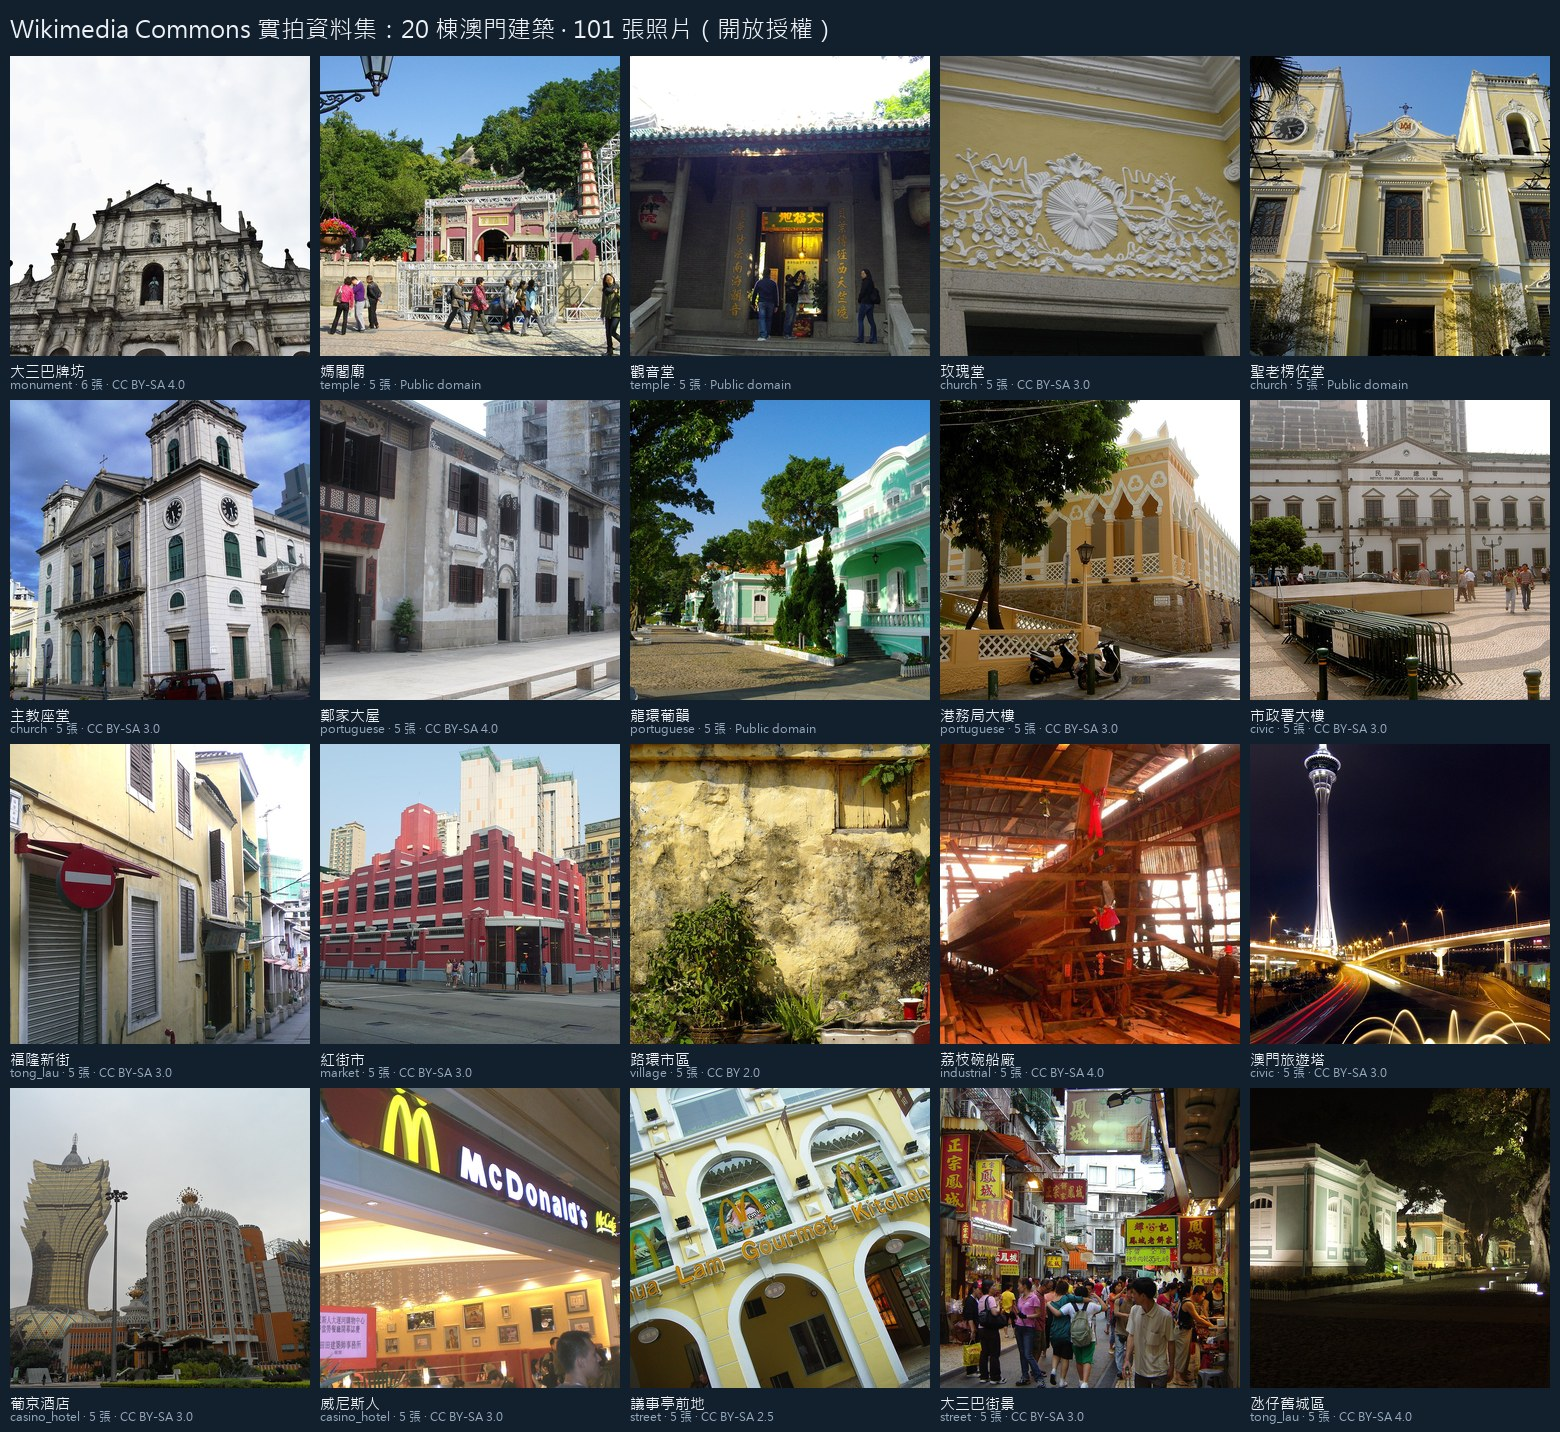
\includegraphics[width=0.94\linewidth]{figs/cc-sheet.jpg}
\caption{真實照片集一覽（每棟建築一張代表影像，含類別與授權）。這批照片是第 4.2 節「真實世界」結果的來源。}
\label{fig:cc-sheet}
\end{figure}

\subsection{自訓資料集的自動預標註}
COCO 預訓練模型沒有「建築」類別，因此我們自建 11 類資料集並以 YOLO-World 開放詞彙偵測預先框出建築位置；類別則直接採用資料夾標籤（\texttt{temple/} 目錄中的影像即為廟宇），因此人工標註只需修正框的位置與大小，不必重新判斷類別，可大幅縮短標註時間。下圖為預標註結果的抽樣檢查。

\begin{figure}[H]
\centering
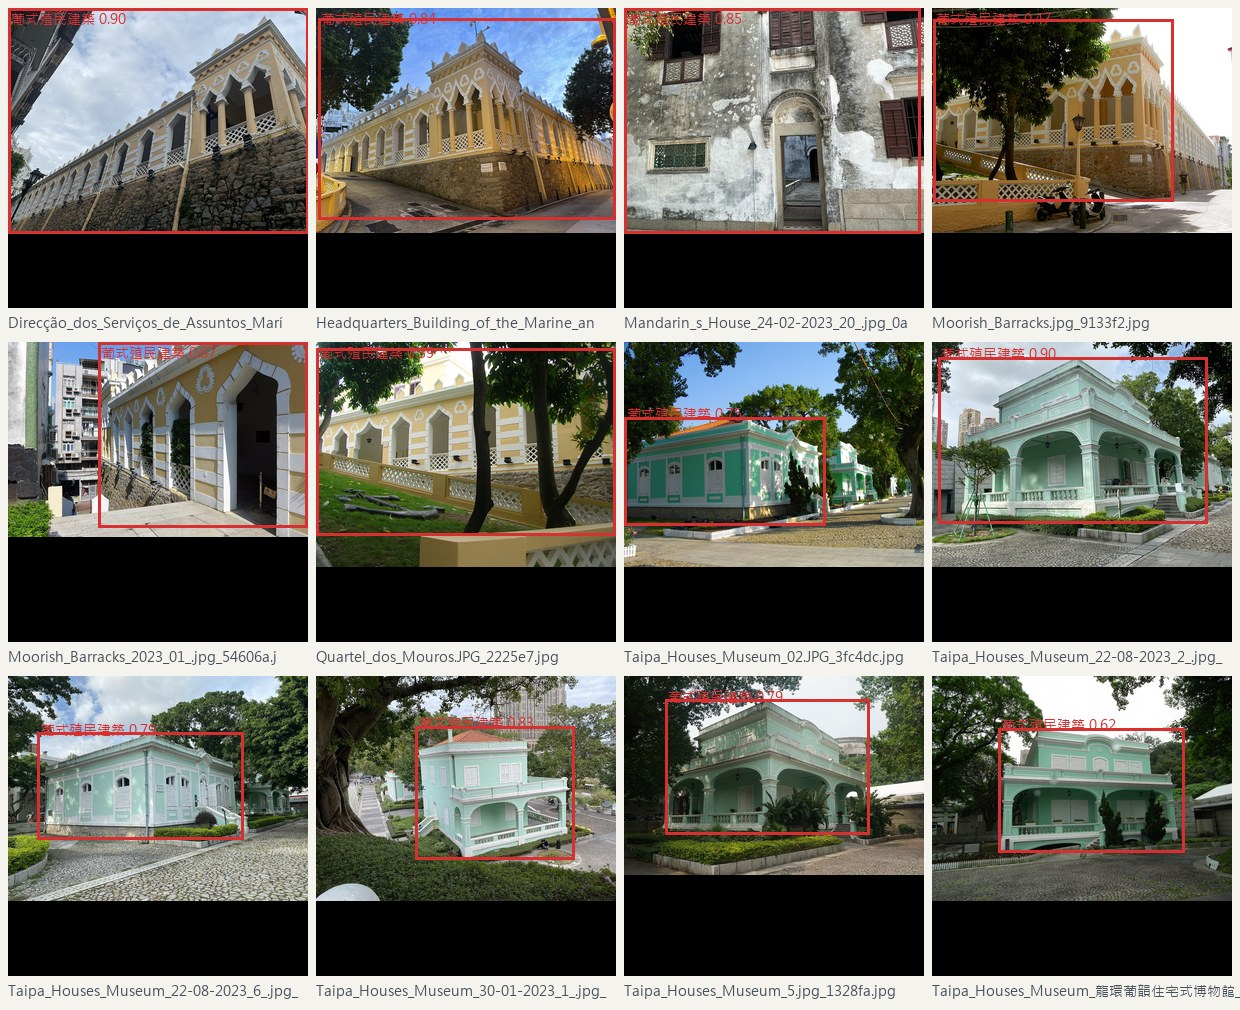
\includegraphics[width=0.88\linewidth]{figs/prelabel.jpg}
\caption{自動預標註結果。框由 YOLO-World 產生、類別由資料夾標籤決定；這是弱標註，人工修正後 mAP 可再提升。}
\end{figure}

\subsection{作品交付清單}
本作品除研究報告外，另包含可直接使用的系統、資料與可重現的評測流程：

\begin{table}[H]
\centering\small
\begin{tabular}{@{}p{3.4cm}p{6.4cm}p{5.5cm}@{}}
\toprule
\textbf{交付項目} & \textbf{內容} & \textbf{位置} \\
\midrule
3D 地圖網站 & 24,904 棟建築量體、地形、61 景點、7 個 3D 模型、導航、圖層、AI 對話與語音 & 線上版 ＋ 可離線本機版 \\
建築記憶點系統 & 拍照歸戶流程、永久編號、時間軸、建築解讀 & \texttt{tools/photo-archive/} \\
重辨識評測 & 兩套資料集、ROC／AUC／閾值掃描、誤判分析、自動報告與圖表 & \texttt{tools/eval/} \\
自訓偵測器 & 11 類澳門建築偵測器（權重檔）＋ 訓練與驗收腳本 & \texttt{tools/yolo-dataset/} \\
即時偵測頁面 & 建築框＋person 框＋人臉模糊，三層同屏、完全離線 & \texttt{live\_detect.py} \\
離線演示頁 & 90 秒五幕演示（拍照 $\rightarrow$ 歸戶 $\rightarrow$ 地圖成點） & \texttt{tools/demo/} \\
A0 展板 & 向量 PDF，數據更新後可一鍵重生成 & \texttt{tools/poster/} \\
吉祥物與標誌 & 「阿獅」三視圖與對話人格、標誌設計需求與配色 & \texttt{tools/mascot/}、\texttt{tools/brand/} \\
資料授權紀錄 & 202 筆影像的作者、授權、日期與來源頁 & 各資料集的 \texttt{ATTRIBUTION.csv} \\
\bottomrule
\end{tabular}
\caption{作品交付清單。所有項目皆可依附錄 A 的指令重新產生。}
\end{table}

\subsection{A0 展板}
展板由 Python 直接產生向量 PDF（A0 直式 841$\times$1189 mm，文字與圖表皆為向量，放大不失真），內容包含研究問題、方法流程、量化結果、資料誠信與限制，右側附作品網址的 QR code。圖表全部由評測腳本自動輸出，因此數據更新後重新執行一次即可同步。

\begin{figure}[H]
\centering
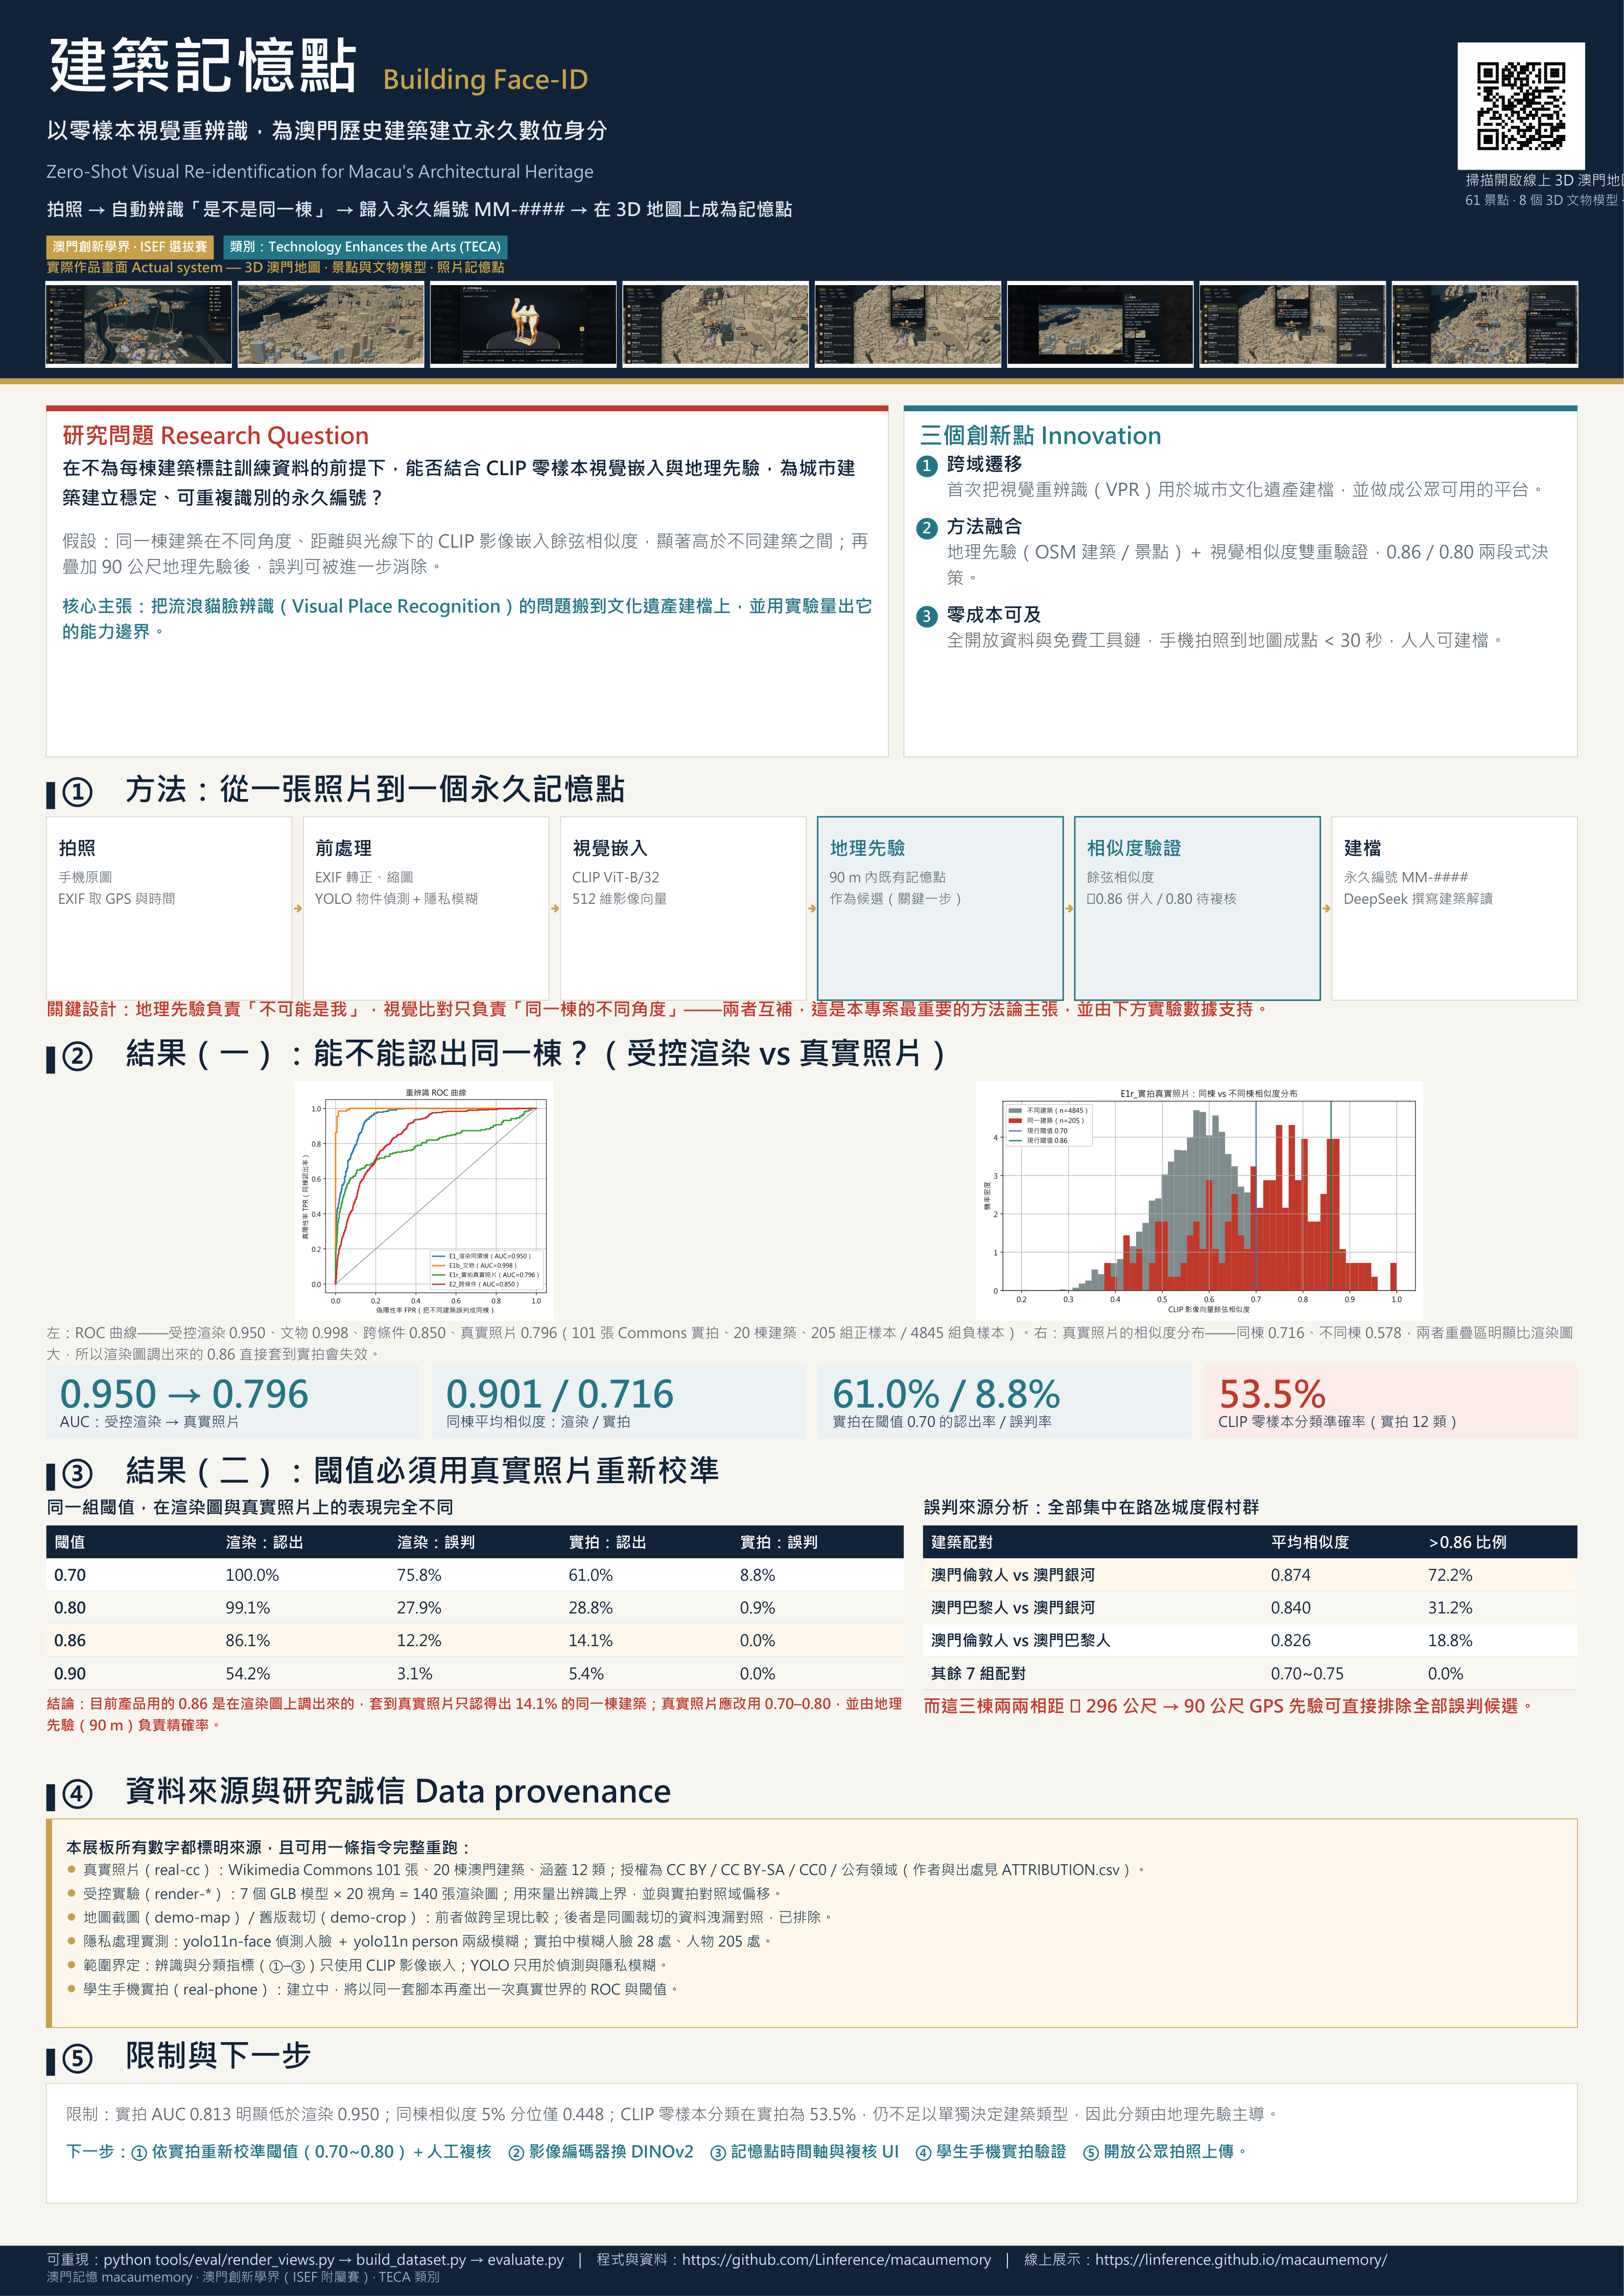
\includegraphics[width=0.62\linewidth]{figs/poster.png}
\caption{A0 展板（可印製；含資料誠信區塊，明確標示渲染圖與實拍照片的來源）。}
\end{figure}

\vspace{0.1cm}
\noindent\textbf{作品網址：}\url{https://linference.github.io/macaumemory/}\\
\textbf{原始碼：}\url{https://github.com/Linference/macaumemory}

\vspace{0.25cm}
\noindent 本作品的全部成果——3D 地圖網站、建築記憶點系統、兩套評測資料集、自訓偵測器與評測腳本、展板與離線演示頁——均公開於上述網址，所有數字皆可依附錄 A 的指令重新產生。我們刻意保留完整的失敗與修正紀錄，因為對一個要被公眾長期使用的文化遺產系統而言，\textbf{可被檢驗與可被修正，比一時的漂亮數字更重要}。

\end{document}
